\noindent

\includegraphics[height=1.25cm]{images/pictograms/benchmark}

\includegraphics[height=1.25cm]{images/pictograms/under_construction}

\includegraphics[height=1.25cm]{images/pictograms/FEM}

\includegraphics[height=1.25cm]{images/pictograms/paraview}


%%%%%%%%%%%%%%%%%%%%%%%%%%%%%%%%%%%%%%%%%%%%%%%%%%%%%%%%%%%%%%%%%%%%%%%%%%%%%%%%%%%%%%%%%%%%%%%%%%%

\begin{flushright} {\tiny {\color{gray} python\_codes/fieldstone\_147/text.tex}} \end{flushright}

\lstinputlisting[language=bash,basicstyle=\small]{python_codes/fieldstone_147/keywords.key}

\par\noindent\rule{\textwidth}{0.4pt}

\begin{center}
\inpython
{\small Code: \url{https://github.com/cedrict/fieldstone/tree/master/python_codes/fieldstone_147}}
\end{center}

\par\noindent\rule{\textwidth}{0.4pt}

%%%%%%%%%%%%%%%%%%%%%%%%%%%%%%%%%%%%%%%%%%%%%%%%%%%%%%%%%%%%%%%%%%%%%%%%%%%%%%%%%%%%%%%%%%%%%%%%%%%

The idea behind this \stone is the comparison of various approaches to solve the 
Stokes system. We here consider simple setups in a 2D rectangular domain. 
The code relies on the \QtwoQone element pair and is based on \stone~\ref{f18}.

In almost all previous stones I have used {\python spsolve} to solve the linear system
but looking online we find that there are many more methods 
available\footnote{\url{https://docs.scipy.org/doc/scipy/reference/sparse.linalg.html}}.
Of all available I highlight the following ones:

\begin{itemize}
\item Direct methods for linear equation systems
\begin{itemize}
\item {\python spsolve}:  
It looks like it is the SuperLU solver\footnote{\url{https://caam37830.github.io/book/02_linear_algebra/sparse_linalg.html}}. 
\item {\python spsolve+UMFPACK}: ({\python solver=11}) 
\end{itemize}
\item Iterative methods for linear equation systems:
\begin{itemize}
\item {\python bicg}(A, b[, x0, tol, maxiter, M, callback, atol]) ({\python solver=9})
\item {\python bicgstab}(A, b[, x0, tol, maxiter, M, ...]) ({\python solver=10})
\item {\python cg}(A, b[, x0, tol, maxiter, M, callback, atol])
\item {\python cgs}(A, b[, x0, tol, maxiter, M, callback, atol])  ({\python solver=12})
\item {\python gmres}(A, b[, x0, tol, restart, maxiter, M, ...]) ({\python solver=2})
\item {\python lgmres}(A, b[, x0, tol, maxiter, M, ...]) ({\python solver=3})
\item {\python minres}(A, b[, x0, shift, tol, maxiter, M, ...]) ({\python solver=5})
\item {\python qmr}(A, b[, x0, tol, maxiter, M1, M2, ...]) ({\python solver=6})
\item {\python gcrotmk}(A, b[, x0, tol, maxiter, M, ...]) ({\python solver=8})
\item {\python tfqmr}(A, b[, x0, tol, maxiter, M, callback, ...]) ({\python solver=7})
\end{itemize}
\end{itemize}

If we build the system as a single (sparse) two-dimensional array 
we can right away rule out {\python cg} which requires 
a SPD matrix\footnote{\url{https://en.wikipedia.org/wiki/Conjugate_gradient_method}}. 
We will then try all the other ones.

Additionally we can build the $\K$ and $\G$ blocks and use conjugate gradient method on 
the Schur complement equation ('SC-CG'), as explained in Section~\ref{MMM-ss:schurpcg}.
This solver is implemented in {\tt schur\_complement\_cg\_solver.py}.
It requires an inner solver called once per iteration on the $\K$ block.
We then have the choice between using a direct solver ({\python solver=4})
or using a conjugate gradient
approach since $\K$ is SPD ({\python solve=13}). 
By using CG we pretty much ensure that memory 
requirements remain very low.
Another variant consists in acknowledging that inside the iterations the 
block $\K$ does not change, so that we can compute its LU decomposition
and use this decomposition every time that we need to solve a linear
system with $\K$. This is {\python solver=14}. 
This option means that the LU factors are stored in the memory longer than in the standard
case but with equal memory use.

All these methods should also be used with a preconditioner, which we will 
investigate later on.

Iterative solver require a tolerance value and it is set to 1e-7 unless mentioned
otherwise.

\newpage

\begin{enumerate}
%-----------------01
\item the first solver is the usual one I use in all the stones
\begin{lstlisting}
   sol=sps.linalg.spsolve(sparse_matrix,rhs,use_umfpack=False)
\end{lstlisting}
%-----------------02
\item the second solver is the gmres from linalg 
\begin{lstlisting}
   sol,info = scipy.sparse.linalg.gmres(sparse_matrix, rhs, restart=2000,tol=tolerance,M=Mprec)
\end{lstlisting}
%-----------------03
\item the third one is the lgmres from linalg
\begin{lstlisting}
   sol = scipy.sparse.linalg.lgmres(sparse_matrix, rhs,atol=1e-16,tol=tolerance)[0]
\end{lstlisting}
%-----------------04
\item the fourth one is my Schur complement CG solver using direct solver for inner solve
\begin{lstlisting}
   solV,p,niter=schur_complement_cg_solver(K_mat,G_mat,M_mat,f_rhs,h_rhs,\
                                          NfemV,NfemP,niter_max,tolerance,use_precond,'direct')
\end{lstlisting}
%-----------------05
\item the fifth one is minres from linalg
\begin{lstlisting}
   sol = scipy.sparse.linalg.minres(sparse_matrix, rhs, tol=1e-10)[0]
\end{lstlisting}
%-----------------06
\item the sixth one is the qmr from linalg
\begin{lstlisting}
   sol = scipy.sparse.linalg.qmr(sparse_matrix, rhs, tol=tolerance)[0]
\end{lstlisting}
%-----------------07
\item the seventh one is the tfqmr from linalg
\begin{lstlisting}
   sol = scipy.sparse.linalg.tfqmr(sparse_matrix, rhs, tol=1e-10)[0]
\end{lstlisting}
%-----------------08
\item the eighth one is the gcrotmk from linalg
\begin{lstlisting}
   sol = scipy.sparse.linalg.gcrotmk(sparse_matrix, rhs,atol=1e-16, tol=1e-10)[0]
\end{lstlisting}
%-----------------09
\item the ninth one is the bicg from linalg
\begin{lstlisting}
   sol = scipy.sparse.linalg.bicg(sparse_matrix, rhs, tol=tolerance)[0]
\end{lstlisting}
%-----------------10
\item the tenth one is bicgstab from linalg
\begin{lstlisting}
   sol = scipy.sparse.linalg.bicgstab(sparse_matrix, rhs, tol=tolerance)[0]
\end{lstlisting}
%-----------------11
\item the eleventh one is spsolve+umfpack 
\begin{lstlisting}
   sol=sps.linalg.spsolve(sparse_matrix,rhs,use_umfpack=True)
\end{lstlisting}
%-----------------12
\item the twelfth one is cgs from linalg
\begin{lstlisting}
   sol = scipy.sparse.linalg.cgs(sparse_matrix, rhs, tol=tolerance)[0]
\end{lstlisting}
%-----------------13
\item the thirteenth one is my Schur complement CG solver using cg for inner solve
\begin{lstlisting}
   solV,p,niter=schur_complement_cg_solver(K_mat,G_mat,M_mat,f_rhs,h_rhs,\
                                           NfemV,NfemP,niter_max,tolerance,use_precond,'cg')
\end{lstlisting}
%-----------------14
\item the fourteenth one is my Schur complement CG solver using splu for inner solve
\begin{lstlisting}
   solV,p,niter=schur_complement_cg_solver(K_mat,G_mat,M_mat,f_rhs,h_rhs,\
                                           NfemV,NfemP,niter_max,tolerance,use_precond,'splu')
\end{lstlisting}
%-----------------15
\item uzawa 1: Section 5.1 \cite{braess}. Parameterised by $\alpha$(=2000 default)
\begin{lstlisting}
   alpha=2000
   solV,p,niter=uzawa1_solver(K_mat,G_mat,M_mat,f_rhs,h_rhs,\
                       NfemV,NfemP,niter_max,tolerance,use_precond,'direct',alpha)
\end{lstlisting}

%-----------------16
\item uzawa 2: Section 5.2 \cite{braess}. 
\begin{lstlisting}
   solV,p,niter=uzawa2_solver(K_mat,G_mat,M_mat,f_rhs,h_rhs,\
                       NfemV,NfemP,niter_max,tolerance,use_precond,'direct')
\end{lstlisting}




\end{enumerate}


\newpage
%====================================================
\section*{Donea \& Huerta mms Without preconditioner}

\begin{center}
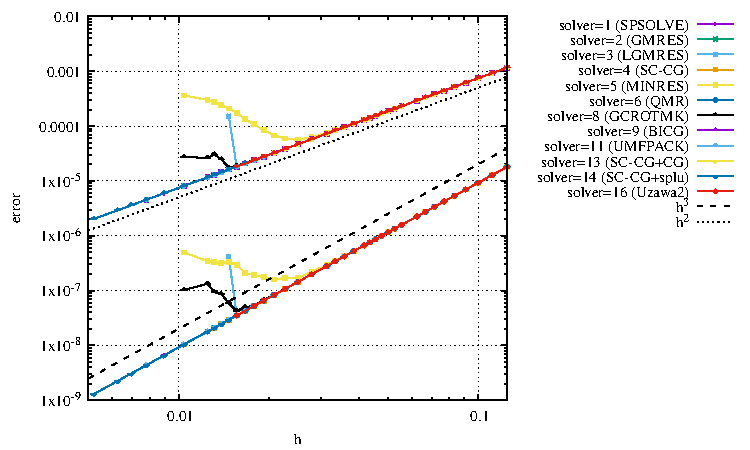
\includegraphics[width=12cm]{python_codes/fieldstone_147/RESULTS/errors.pdf}
\end{center}

\begin{center}
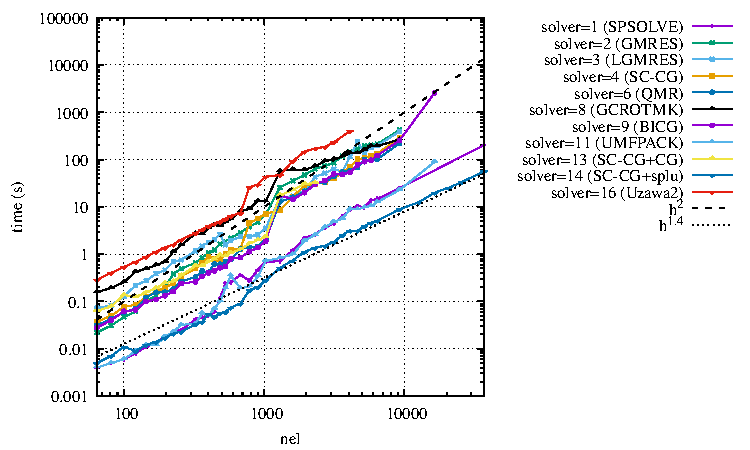
\includegraphics[width=12cm]{python_codes/fieldstone_147/RESULTS/solve.pdf} \\
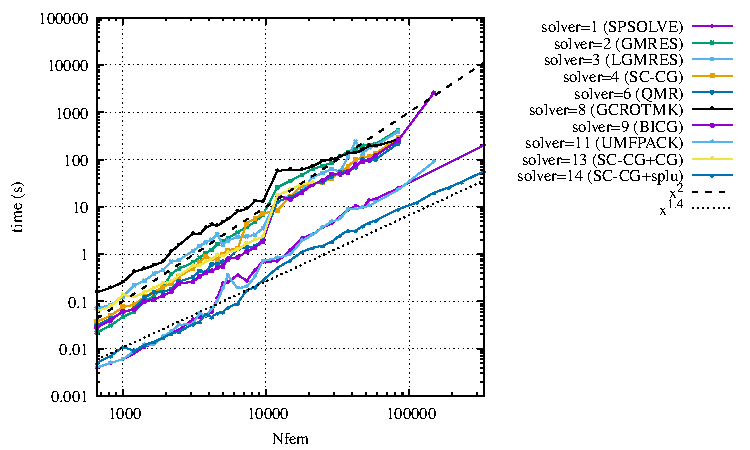
\includegraphics[width=12cm]{python_codes/fieldstone_147/RESULTS/solve2.pdf}\\
{\captionfont Time to solve linear system. Only results for usable solvers are shown. 
Left: time as a function of the number of elements; Right: 
time as a function of the total number of dofs.}
\end{center}

\begin{center}
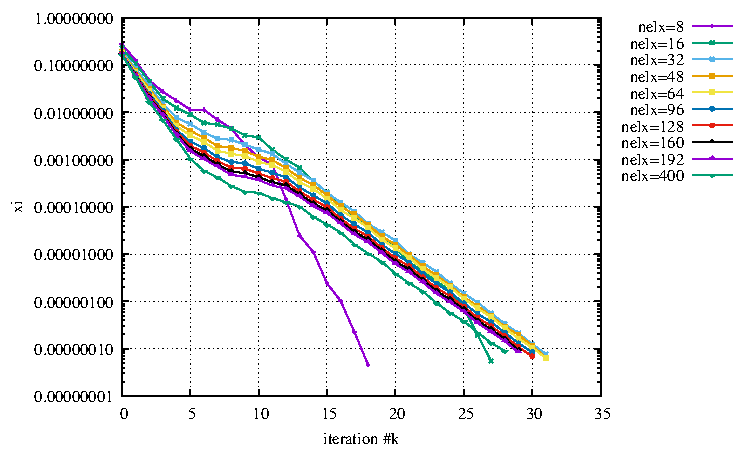
\includegraphics[width=12cm]{python_codes/fieldstone_147/RESULTS/convergence_schur_cpl.pdf}\\
{\captionfont Convergence of the SC-CG solver as function of resolution.}
\end{center}

On the following figure I plot the velocity and pressure errors for SC-CG+ilu solver 
for different values of the relative tolerance. We find that the solve time is not 
much influenced by the tolerance, but unsurprisingly the accuracy of the solution is: 
\begin{center}
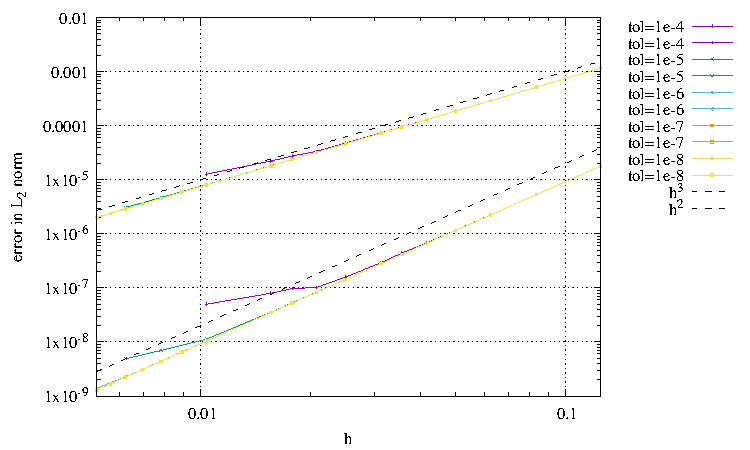
\includegraphics[width=8cm]{python_codes/fieldstone_147/RESULTS/tol_study_solver14/errors.pdf}
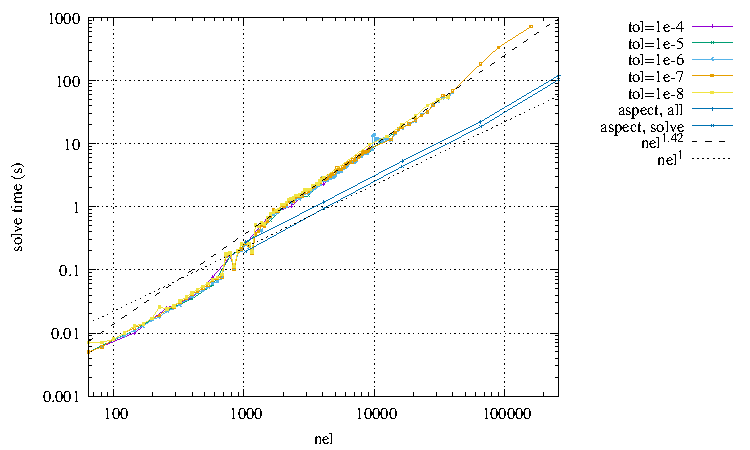
\includegraphics[width=8cm]{python_codes/fieldstone_147/RESULTS/tol_study_solver14/solve.pdf}\\
{\captionfont Left: Influence of the relative tolerance on the accuracy of the solution obtained 
with the SC-CG+ilu ({\python solver=14}). Right: solve time in seconds.}
\end{center}
It appears that a relative tolerance of $10^{-6}$ is enough, but I set it to $10^{-7}$ default
to be on the safe side (when looking closley at high resolution it looks like the 
blue curve of $10^{-6}$  seems to separate from the orange one from $10^{-7}$).

I have also run \aspect on the same problem (with the same type of elements) and on only 
1 core (while the spsolve inner solve tends to use all available cores of my laptop). 
Since \aspect reports the assembly time, the preconditioner time and the solve
time separately I add them together.
We find that the solver outperforms mine (obviously!) and more importantly that 
is scales linearly with the number of elements. 
The highest resolutions so far are $300\times 300$ elements and the memory requirements 
were about half of my laptop RAM, so about 16Gb, and $400\times 400$ which requires
about 20+ Gb.


We can also look at the $L_2$ error on the velocity divergence:

\begin{center}
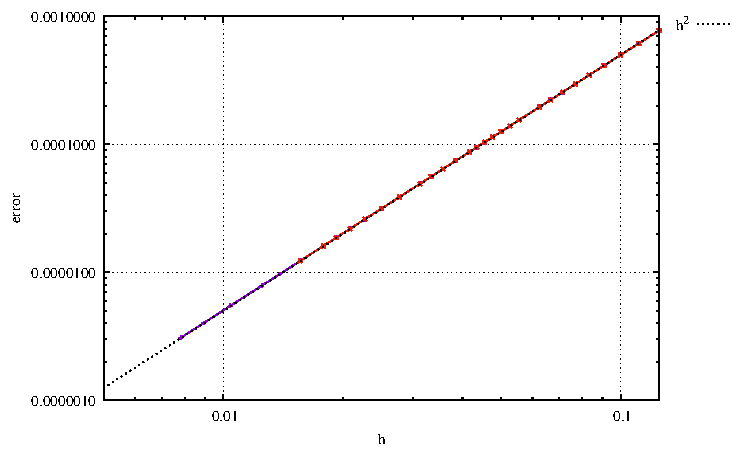
\includegraphics[width=8cm]{python_codes/fieldstone_147/RESULTS/error_divv.pdf}
\end{center}

\newpage
%......................................
\subsubsection*{About the Uzawa solvers}

U1 is uzawa of Braess, section 5.1: simple to implement but a parameter is needed. 
U2 is uzawa of Braess, section 5.2
U3 is conjugate gradient on schur complement, section 5.3.

The three algorithms U1, U2, U3 are reproduced from \cite{braess} hereunder from left to right for convenience:
\begin{center}
\fbox{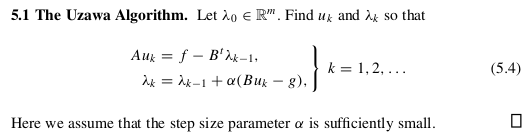
\includegraphics[width=5.6cm]{python_codes/fieldstone_147/images/braess_U1}}
\fbox{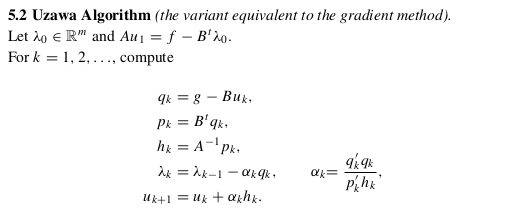
\includegraphics[width=5.6cm]{python_codes/fieldstone_147/images/braess_U2}}
\fbox{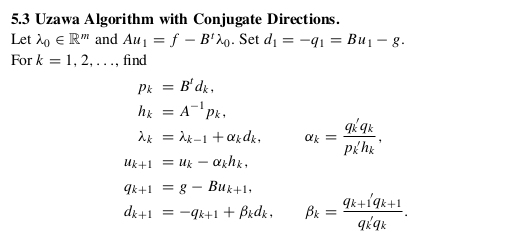
\includegraphics[width=5.6cm]{python_codes/fieldstone_147/images/braess_U3}}\\
Taken from \textcite{braess}.
\end{center}

The following figure shows the convergence of this solver for different values of this parameter.
20000 makes the solver explode.	

\begin{center}
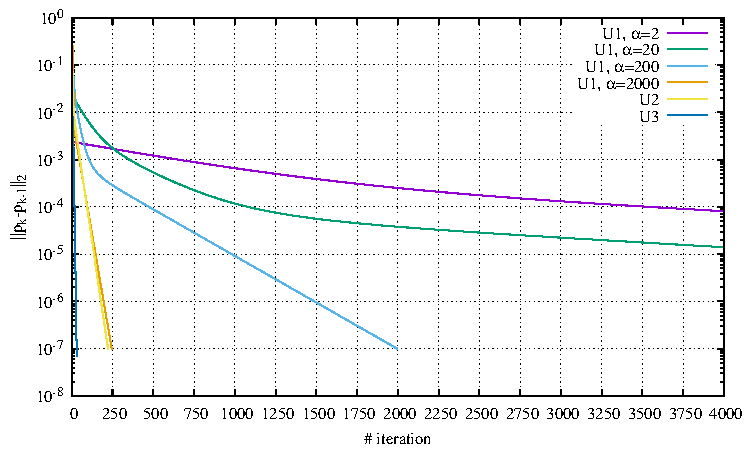
\includegraphics[width=8cm]{python_codes/fieldstone_147/RESULTS/uzawa123/convergence_24x24.pdf}
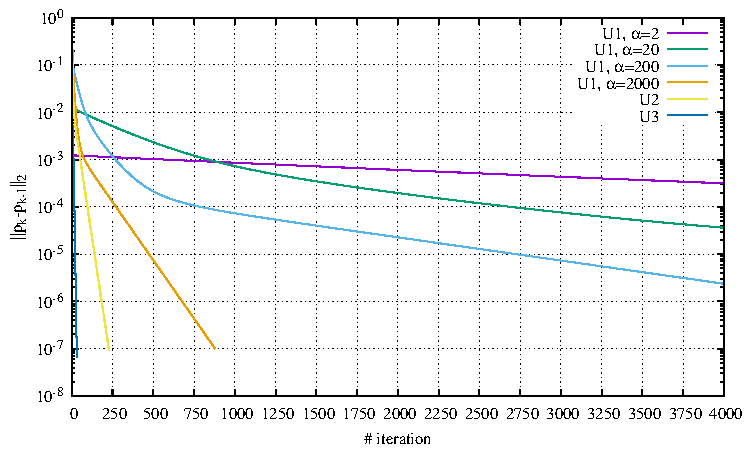
\includegraphics[width=8cm]{python_codes/fieldstone_147/RESULTS/uzawa123/convergence_48x48.pdf}\\
{\captionfont Convergence on 24x24 mesh (left) and 48x48 mesh (right) 
for Donea \& Huerta manufactured solution.}
\end{center}

We see that the $\alpha$ parameter should be a function of resolution, and that 
the uzawa2 converges in the same number of iterations because it automatically 
computes the step.


Actually when focusing now on U2 and U3 only and running the experiment at increasing resolutions I find ({\it as expected for stable element pairs}) that the number of iterations is independent of the resolution:
\begin{center}
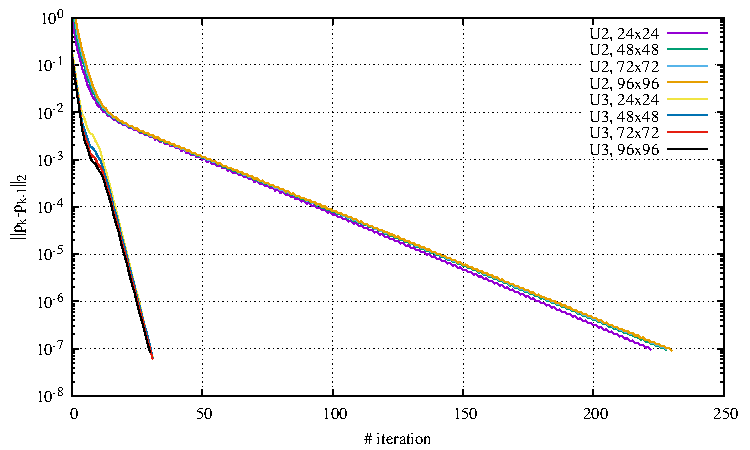
\includegraphics[width=8cm]{python_codes/fieldstone_147/RESULTS/uzawa123/convergence_uzawa23}
\end{center}



This shows that\\
1) U2 is a much better/safe algorithm than U1 while being equally simple to implement, thereby proving that U1
 should be discarded altogether; \\
2) U3 is the obvious starting point if one wishes to offer an improvement on Uzawa-type solvers as it is by far the best of the three and is marginally more complex to implement than U1 or U2.






\newpage
%-------------------------
\subsection*{Conclusions}

\begin{itemize}
\item direct method spsolve about 10x faster than all others (except solver 14!)
\item UMFPACK option in spsolve does not yield substantial differences
\item my own Schur complement CG solver rivals other LINALG solvers (solver 4, 13) ! 
\item MINRES, even with very low tolerance 1e-10, ultimately fails
\item LGMRES seems to work fine, very similar to GMRES but does not always converge.
\item TFQMR, BICGSTAB, CGS are out: they fail to converge and/or return 
very wrong results
\item GCROTMK usable but slowest, also fails at high resolution 
\item number of iterations of SC-CG is independent of resolution, as expected
from a stable element pair (for isoviscous flow)
\item solve time for iterative method rather comparable, no clear best
\item SC-CG with direct or cg inner solve are comparable in terms of 
solve time. There is still something wrong about my having to 
set tol of cg extremely low, and even then it ends up crashing at nel=52 ...
\item my own SC-CG+ilu is faster than spsolve!
\end{itemize}

In the end, I keep SPSOLVE, SC-CG, GMRES, QMR, BICG.

\newpage
%====================================================
\section*{Donea \& Huerta mms With preconditioner}

Following this site\footnote{\url{https://caam37830.github.io/book/02_linear_algebra/sparse_linalg.html}}
we build an ILU preconditioner as follows:
\begin{lstlisting}
ILUfact = sla.spilu(sparse_matrix)
M = sla.LinearOperator(
    shape = sparse_matrix.shape,
    matvec = lambda b: ILUfact.solve(b))
\end{lstlisting}
However, I find that the preconditioner does not work with gmres, minres, cg, ...

This means that I need to build my own preconditioner. 
For the SC-CG 

We have designed X preconditioners:
\begin{itemize}
\item {\tt precond\_type=0} It is the unit matrix (so it does nothing). 
%\item {\tt precond\_type=1} This is a very simple one as it is
%diagonal and built element by element:
%\[
%M_{e,e} = \frac{h_x h_y}{\eta_e} 
%\]
%where $e$ is an element and $\eta_e$ the viscosity evaluated in its center. Note that 
%averages based on quadrature point values could also be considered (or any other kind of projection).

\item {\tt precond\_type=2}
\[
{\bm M} = \G^T (diag [\K]  )^{-1} \G 
\]
\item {\tt precond\_type=3} 
\[
{\bm M} = diag \left[ \G^T (diag [\K]  )^{-1} \G \right]
\]
\item {\tt precond\_type=4} Same as 2, but instead of using the 
diagonal of $ \G^T (diag [\K]  )^{-1} \G$ we lump the matrix instead.

\end{itemize}

{\Large unfinished}



%%%%%%%%%%%%%%%%%%%%%%%%%%%%%%%%%%%%%%%%%%%%%%%%%%%%%%%%%%%%%%%%%%%%%%%%%%%%%%%%%%%%%%%%%%%%%%%%%%%
\par\noindent\rule{\textwidth}{0.4pt}

\vspace{.5cm}

\begin{center}
\fbox{\begin{minipage}{0.9\textwidth}
{\color{teal}To Do, open questions, future work?}
\begin{itemize}
\item do smthg
\end{itemize}
\end{minipage}}
\end{center}

%%%%%%%%%%%%%%%%%%%%%%%%%%%%%%%%%%%%%%%%%%%%%%%%%%%%%%%%%%%%%%%%%%%%%%%%%%%%%%%%%%%%%%%%%%%%%%%%%%%
\vspace{.5cm}

\Literature:\\
\fullcite{xxxxYY}







